\documentclass[10pt,a4paper]{amsart}
\usepackage[margin=19mm]{geometry}
\usepackage{amsmath,amssymb,mathtools}
\usepackage[scr=rsfs,cal=euler]{mathalfa}
\usepackage{xfrac}
\usepackage[unicode,hidelinks,bookmarks=false]{hyperref}
\newcommand{\ie}{i.e.\ }
\newcommand{\cf}{cf.\ }
\newcommand{\resp}{respectively\ }
\newcommand{\Subsection}{\subsection}
\providecommand{\nobreakdash}{\nobreak\hbox{-}}
\setlength{\emergencystretch}{2em}
\multlinegap0pt
\usepackage{tikz}
\usepackage{amssymb}
\usepackage{float}
\usepackage{mathtools}
\usepackage{csquotes}
\usepackage[shortlabels]{enumitem}
\newtheorem{lemma}{Lemma}
\newtheorem{proposition}{Proposition}
\newtheorem{scope}{Scope}
\title{Network Realignment Complexes over General Graphs}
\author{Fabienne Klatt, Iason Papadopoulos, Marc Raffelsiefen}
\date{Source: arXiv:2607.07404v1 (CC BY 4.0)}
\begin{document}
\maketitle

\noindent\emph{Source and licence.} Network Realignment Complexes over General Graphs. Version arXiv:2607.07404v1 (CC BY 4.0), distributed by arXiv under the Creative Commons Attribution 4.0 International licence, http://creativecommons.org/licenses/by/4.0/, as recorded in the arXiv licence metadata for this exact version and shown on the abstract page https://arxiv.org/abs/2607.07404v1. Full licence notice: \texttt{licenses/arxiv-2607.07404-CC-BY-4.0.txt}.\par\smallskip

\noindent\textit{Editorial scope.} Counted unit: the article's proposition prop:FourCycleCompletion (source0.tex lines 2513--2515). The article's complete original proof of it is delivered with it (source0.tex lines 2551--2686, one \texttt{proof} environment of 136 lines, which the article places away from the statement). No mathematics is written, repaired or re-derived: the statement and the proof are the article's own lines, in the article's own notation, and no retained line is substituted or re-flowed.  Retained uncounted as the source-local context the proof needs: lines 1716--1734; lines 2533--2539.  Nothing was omitted from any retained span, so the package carries no omission record.  No retained line contains a citation, so the wrapper carries no bibliography and no bibliography entry.  The retained lines contain the article's own diagram code, which the wrapper typesets with the standard tikz packages; no image file is delivered and the package declares no asset dependency.  Editorial formatting only, in addition: an AMS \texttt{amsart} preamble that restates the article's own declarations and macros used by the retained lines, namely the environments \texttt{lemma}, \texttt{proposition}, \texttt{scope} on separate counters, together with the standard packages those lines need.  The retained environments print in this document as Lemma 1, Proposition 1, Scope 1 in order of appearance, whereas the article prints the same items with the numbering of its own full document.  The complete native source of the article as distributed in the arXiv e-print for this exact version is bundled unchanged as \texttt{sources/204705/source0.tex}.
\begin{lemma}\label{iter}
	Let $N = (T,r)$ be a 1-dimensional realignment (i.e. leaf slide). We write $B = \{v\}$ and  $r(v) = (u,w)$. Let $c\in V(T) = [n]\setminus\{v\}$.

	In this situation, the leaf slide changes the values of $\Psi$ by at most one. To be precise, we have
	\begin{equation}\label{Psiiter}
		\begin{split}
			|\Psi(N^{v\to u})-\Psi(N^{v\to w})|&  = 1\text{, if $n$ is even, and}\\
			|\Psi(N^{v\to u})-\Psi(N^{v\to w})|&  \leq 1\text{, if $n$ is odd.}
		\end{split}
	\end{equation}
	The behaviour of $\Phi$ depends on whether the slide is performed towards or away from $c$. Let $\gamma$ be the unique path connecting $w$ and $c$ in $T$, then
	\begin{equation}\label{Phiiter}
		\Phi_c(N^{v\to u}) = 
		\begin{cases}
			\Phi_c(N^{v\to w}) - 1, &\text{if $u$ lies on $\gamma$,}\\
			\Phi_c(N^{v\to w}) + 1, &\text{otherwise.}\\
		\end{cases}
	\end{equation}
\end{lemma} 

		\begin{lemma} \label{lem:MaxComponentLeafSlide}
			Let $T$ be a tree and $c$ a centroid of $T$. Let $v$ be a leaf of $T$ with $p_T(v) \neq c$. Denote by $u_v$ the vertex adjacent to $p_T(v)$ along the unique path from $p_T(v)$ to $c$. Then
			\[
				F_\mathrm{cent}(T) - 1 \leq F_\mathrm{cent}(T^{v\rightsquigarrow u_v}) \leq F_\mathrm{cent}(T).
			\]
			Moreover, $F_\mathrm{cent}(T^{v\rightsquigarrow u_v}) = F_\mathrm{cent}(T)$, whenever $u_v \neq c$.
		\end{lemma}

		\begin{proposition} \label{prop:FourCycleCompletion}
			Let $H$ be a subgraph of $\mathcal{G}_n$ that is closed under 4-cycle completion. If $\Sigma_n \subseteq H$, then $H = \mathcal{G}_n$.
		\end{proposition}

		\begin{proof} [Proof of \autoref{prop:FourCycleCompletion}]
			It suffices to show that for any proper subgraph $H\subset \mathcal{G}_n$ with $\Sigma_n \subseteq H$ there exists a 4-cycle $C$ with $|V(C) \cap V(H)| = 3$. This proves that $H$ is not closed under 4-cycle completion.

			Let $T\in \mathcal{G}_n\setminus H$ that minimises $\Psi(T) - F_\mathrm{cent}(T)$, and among all such trees, minimises $\Psi(T)$. 

			\textbf{Case 1:} $T$ has a centroid $c$ and two leaves $v,w$ with $p_T(v) \neq c \neq p_T(w)$.\\
			Let $u_v$ and $u_w$ denote the vertices adjacent to $p_T(v)$ and $p_T(w)$ on the unique paths from $p_T(v)$ to $c$ and from $p_T(w)$ to $c$, respectively. Set
			\[
				T_1 = T^{v\rightsquigarrow u_v}, \quad T_3 = T^{w\rightsquigarrow u_w}, \quad \text{and} \quad T_2 = T_1^{w\rightsquigarrow u_w} = T_3^{v\rightsquigarrow u_v}.
			\]
			By Lemmas \ref{iter} and \ref{lem:MaxComponentLeafSlide}, $\Psi(T_i) - F_\mathrm{cent}(T_i) \leq \Psi(T) - F_\mathrm{cent}(T)$ and $\Psi(T_i) < \Psi(T)$ for $1\leq i \leq 3$. Hence, $T_1, T_2, T_3\in H$. Therefore, the 4-cycle $C = T, T_1, T_2, T_3, T$ satisfies $|V(C) \cap V(H)| = 3$.

			\textbf{Case 2:} For every centroid $c$ of $T$, at most one leaf $v$ satisfies $p_T(v) \neq c$.\\
			Suppose $T$ has two centroids. Then $T$ has at most two leaves each connected to a centroid. Thus, $|V(T)| \leq 4$, contradicting $T\notin \Sigma_n\subseteq H$. 
			
			Let $c_1$ denote the single centroid of $T$. Since $T\notin \Sigma_n$, there exists a leaf $v$ such that $d_T(v,c_1) \geq 3$. Let $c_2$ denote the vertex adjacent to $c_1$ along the unique path from $c_1$ to $v$. Let $c_2, v_1,\ldots, v_k$ denote the neighbours of $c_1$. Set
			\[
				T_0 = T \quad \text{and} \quad T_i = T_{i-1}^{v_i\rightsquigarrow c_2} \quad \text{for } 1\leq i\leq k.
			\]
			\autoref{fig:FourCycleCompletion} shows the trees $T, T_i$ and $T_k$ of the above sequence for a path from $c_1$ to $v$ of length 3. 
			% Figure depicts the involved trees in Case 2.2
			%-----------------------------------------------------------------
			\begin{figure}[tbp]
				\centering
				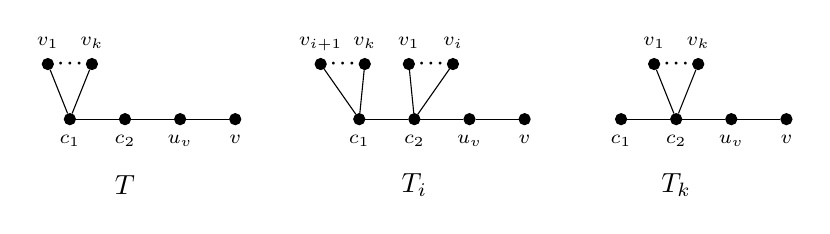
\begin{tikzpicture}[dot/.style={circle, draw, fill, inner sep=0pt, minimum size=4pt}]

					\newcommand{\diagramScale}{0.7}

					\begin{scope}[scale=\diagramScale]
						% vertices
						\node[dot, label={below:{\scriptsize $c_1$}}] (u1) at (0,0) {};
						\node[dot, label={below:{\scriptsize $c_2$}}] (u2) at (1,0) {};
						\node[dot, label={below:{\scriptsize $u_v$}}] (u3) at (2,0) {};
						\node[dot, label={below:{\scriptsize $v$}}] (u4) at (3,0) {};
						\node[dot, label={above:{\scriptsize $v_1$}}] (u5) at (-.4,1) {};
						\node[dot, label={above:{\scriptsize $v_k$}}] (u6) at (.4,1) {};
						\node at (0,1) {$\cdot\!\cdot\!\cdot$};
						\node at (1,-1.2) {$T$};
						% arrows
						\draw (u1) -- (u2) -- (u3) -- (u4);
						\draw (u5) -- (u1) -- (u6);
					\end{scope}

					\begin{scope}[scale=\diagramScale, xshift = 5.25cm]
						% vertices
						\node[dot, label={below:{\scriptsize $c_1$}}] (v1) at (0,0) {};
						\node[dot, label={below:{\scriptsize $c_2$}}] (v2) at (1,0) {};
						\node[dot, label={below:{\scriptsize $u_v$}}] (v3) at (2,0) {};
						\node[dot, label={below:{\scriptsize $v$}}] (v4) at (3,0) {};
						\node[dot, label={[yshift=-.8pt] above:{\scriptsize $v_{i+1}$}}] (v5) at (-.7,1) {};
						\node[dot, label={above:{\scriptsize $v_k$}}] (v6) at (.1,1) {};
						\node[dot, label={above:{\scriptsize $v_1$}}] (v7) at (.9,1) {};
						\node[dot, label={above:{\scriptsize $v_i$}}] (v8) at (1.7,1) {};
						\node at (-.3,1) {$\cdot\!\cdot\!\cdot$};
						\node at (1.3,1) {$\cdot\!\cdot\!\cdot$};
						\node at (1,-1.2) {$T_i$};
						% arrows
						\draw (v1) -- (v2) -- (v3) -- (v4);
						\draw (v5) -- (v1) -- (v6);
						\draw (v7) -- (v2) -- (v8);
					\end{scope}

					\begin{scope}[scale=\diagramScale, xshift = 10cm]
						% vertices
						\node[dot, label={below:{\scriptsize $c_1$}}] (w1) at (0,0) {};
						\node[dot, label={below:{\scriptsize $c_2$}}] (w2) at (1,0) {};
						\node[dot, label={below:{\scriptsize $u_v$}}] (w3) at (2,0) {};
						\node[dot, label={below:{\scriptsize $v$}}] (w4) at (3,0) {};
						\node[dot, label={above:{\scriptsize $v_1$}}] (w5) at (.6,1) {};
						\node[dot, label={above:{\scriptsize $v_k$}}] (w6) at (1.4,1) {};
						\node at (1,1) {$\cdot\!\cdot\!\cdot$};
						\node at (1,-1.2) {$T_k$};
						% arrows
						\draw (w1) -- (w2) -- (w3) -- (w4);
						\draw (w5) -- (w2) -- (w6);
					\end{scope}
				\end{tikzpicture}
				\vspace{-3mm}
				\caption{If the tree $T$ minimises the quantity $\Psi$, then there is no 4-cycle containing $T$ whose other three vertices take strictly lower value in $\Psi$. In this situation, we can construct a sequence $T,T_1,\ldots, T_k$ to find a different tree $T_i$ and a desired 4-cycle. Along this sequence, $\Psi - F_\mathrm{cent}$ never increases.}
				\label{fig:FourCycleCompletion}
			\end{figure}
			%-----------------------------------------------------------------
			
			We claim that $\Psi(T_{i+1}) - F_\mathrm{cent} (T_{i+1}) \leq \Psi(T_i) - F_\mathrm{cent} (T_i)$ for $0\leq i \leq k-1$. By construction, the maximal connected component of $T_i\setminus \{c_1\}$ always contains all vertices except $c_1$ and $v_{i+1},\ldots, v_k$. Hence,
			\[
				F_{c_1} (T_i) = n-k+i-1.
			\]
			Meanwhile, the maximal connected component of $T_i\setminus c_2$ contains either $c_1$ together with $v_{i+1},\ldots, v_k$ or the unique path from $c_2$ to $v$ with $c_2$ removed. Therefore, 
			\[
				F_{c_2} (T_i) = \max \{ k-i+1, \, n-k-2 \}
			\]
			for all $i$. Further, for every $w \neq c_1,c_2$, the sizes of the connected components of $T_i\setminus \{w\}$ and $T\setminus \{w\}$ agree. Since $w$ is not a centroid of $T$, it is not a centroid of $T_i$ either. Hence, we distinguish the following three cases.

			If $c_1$ is a centroid of both $T_i$ and $T_{i+1}$, then 
			\[
				F_{c_1} (T_{i+1}) = n - k + i = F_{c_1} (T_i) + 1,
			\]
			and by \autoref{iter} we have
			\[
				\Psi(T_{i+1}) = \Phi_{c_1}(T_{i+1}) = \Phi_{c_1} (T_i) + 1 = \Psi(T_i) + 1.
			\]
			Therefore, 
			\[
				\Psi(T_{i+1}) - F_\mathrm{cent} (T_{i+1}) = \Psi(T_i) - F_\mathrm{cent} (T_i).
			\]
			If $c_2$ is a centroid of both $T_i$ and $T_{i+1}$, then 
			\[
				\Psi(T_{i+1}) = \Phi_{c_2}(T_{i+1}) = \Phi_{c_2} (T_i) - 1 = \Psi(T_i) - 1
			\]
			by \autoref{iter}. Further, the value of $F_\mathrm{cent}$ changes along a leaf slide by at most one. Hence, 
			\[
				\Psi(T_{i+1}) - F_\mathrm{cent} (T_{i+1}) \leq \Psi(T_i) - F_\mathrm{cent} (T_i).
			\]
			It remains to assume that $c_1$ is only a centroid of $T_i$ and $c_2$ is only a centroid of $T_{i+1}$. Since $c_1$ is not a centroid of $T_{i+1}$, it follows that $\frac{n}{2} < F_{c_1}(T_{i+1}) = n-k+i$. Further, $\frac{n}{2} < F_{c_2}(T_i) = k-i+1$, since $c_2$ is not a centroid of $T_i$ and $n-k-2 \leq \frac{n}{2}$, as $c_2$ is not a centroid of $T$. Combining these two inequalities yields
			\[
				\frac{n}{2} - 1 < k-i < \frac{n}{2}.
			\]
			It follows that $n$ is odd and $k-i = \frac{n-1}{2}$. Hence, $F_{c_1}(T_i) = \frac{n-1}{2} = F_{c_2}(T_{i+1})$ and $\Psi(T_i)-\Psi(T_{i+1}) = \sigma_{T_i}(c_1,c_2) - \sigma_{T_{i+1}}(c_1,c_2) = 0$. Therefore,
			\[
				\Psi(T_{i+1}) - F_\mathrm{cent} (T_{i+1}) = \Psi(T_i) - F_\mathrm{cent} (T_i).
			\]

			Now, it suffices to show that $\Psi(T) > \Psi(T_k)$ to prove that $T_k\in H$. Since each leaf $v_1,\ldots,v_k$ was realigned along the edge $e = (c_1, c_2)$, we have $\sigma_T (\tilde{e}) = \sigma_{T_k} (\tilde{e})$ for all edges $\tilde{e}\neq e$. Hence,
			\[
				\Psi(T) - \Psi(T_k) = \sigma_T (e) - \sigma_{T_k} (e) = d_T(v,c_1) - 1 > 0,
			\]
			Therefore, since $T\notin H$ and $T_k\in H$, there must exist $0\leq i \leq k-1$ such that $T_i\notin H$ and $T_{i+1}\in H$. Let $u_v$ denote the vertex adjacent to $p_T(v)$ on the unique path from $p_T(v)$ to $c_1$. Set
			\[
				S_i = T_i^{v\rightsquigarrow u_v} \quad \text{and} \quad S_{i+1} = T_{i+1}^{v\rightsquigarrow u_v}.
			\]
			If $u_v = c_2$, then $S_i$ and $S_{i+1}$ are weak double star trees, and hence $S_i, S_{i+1} \in \Sigma_n \subseteq H$. Otherwise, $u_v$ is not a centroid, and thus we get 
			\[
				\Psi(T) - F_\mathrm{cent} (T) \geq \Psi(T_j) - F_\mathrm{cent} (T_j) > \Psi(S_j) - F_\mathrm{cent} (S_j)
			\] 
			for $j = i, i+1$ using Lemmas \ref{iter} and \ref{lem:MaxComponentLeafSlide}. Again, the trees $S_i, S_{i+1}$ are contained in $H$. Therefore, $C = T_i, S_i, S_{i+1}, T_{i+1},, T_i$ is a 4-cycle with $|V(C) \cap V(H)| = 3$.
		\end{proof}

\end{document}
